%; whizzy chapter
% -initex iniptex -latex platex -format platex -bibtex jbibtex -fmt fmt
% 以上 whizzytex を使用する場合の設定。


%     Tokyo Debian Meeting resources
%     Copyright (C) 2007 Junichi Uekawa

%     This program is free software; you can redistribute it and/or modify
%     it under the terms of the GNU General Public License as published by
%     the Free Software Foundation; either version 2 of the License, or
%     (at your option) any later version.

%     This program is distributed in the hope that it will be useful,
%     but WITHOUT ANY WARRANTY; without even the implied warranty of
%     MERCHANTABILITY or FITNESS FOR A PARTICULAR PURPOSE.  See the
%     GNU General Public License for more details.

%     You should have received a copy of the GNU General Public License
%     along with this program; if not, write to the Free Software
%     Foundation, Inc., 51 Franklin St, Fifth Floor, Boston, MA  02110-1301 USA

%  preview (shell-command (concat "xpdf " (replace-regexp-in-string "tex$" "pdf"(buffer-file-name)) "&"))
% 画像ファイルを処理するためにはebbを利用してboundingboxを作成。
%(shell-command "cd image200701; ebb *.png")

%%ここからヘッダ開始。

\documentclass[mingoth,a4paper]{jsarticle}
\usepackage[dvipdfmx]{graphicx}
\usepackage{fancybox}
\usepackage{longtable}
\usepackage{ascmac}	% 囲み (screen,itembox)
\usepackage{fancyvrb}   % 囲み Verbatim のために必要
\usepackage[dvipdfmx]{hyperref}
\usepackage{url}
\usepackage[dvipdfmx]{color}
\usepackage{nextpage}

% 日付を定義する、毎月変わります。
\newcommand{\debmtgyear}{2007}
\newcommand{\debmtgdate}{17}
\newcommand{\debmtgmonth}{2}
\newcommand{\debmtgnumber}{25}



%http://www.naney.org/diki/dk/hyperref.html
%日本語EUC系環境の時
\AtBeginDvi{\special{pdf:tounicode EUC-UCS2}}
%シフトJIS系環境の時
%\AtBeginDvi{\special{pdf:tounicode 90ms-RKSJ-UCS2}}

%% spacing の設定をする。外枠を減らす。
\setlength\headheight{0mm}
\setlength\topmargin{-20mm}
\setlength\headsep{0mm}
\setlength\topskip{3mm}
\setlength\maxdepth{4pt}
\setlength\columnsep{6mm}
\setlength\textheight{252mm}
\setlength\topmargin{-5mm}
\setlength\textwidth{170mm}
\setlength\oddsidemargin{-5mm}
\setlength\evensidemargin{-5mm}

% commandline環境を定義。画面入出力についてはcommandline環境
% で表記する
\newenvironment{commandline}%
{\VerbatimEnvironment
  \begin{Sbox}\begin{minipage}{15cm}\begin{fontsize}{7.3}{7.3} \begin{BVerbatim}}%
{\end{BVerbatim}\end{fontsize}\end{minipage}\end{Sbox}
  \setlength{\fboxsep}{8pt}\fbox{\TheSbox}}


%%% start of santaku
\makeatletter
\newwrite\tf@jqz
\immediate\openout\tf@jqz\jobname.jqz\relax
\makeatother
\newcounter{santakucounter}
\newcommand{\santaku}[5]{%
\addtocounter{santakucounter}{1}

\addtocontents{jqz}{\arabic{santakucounter}. #5\\}
\begin{minipage}{1\hsize}
問題\arabic{santakucounter}. 
#1\\
□ A #2\\
□ B #3\\
□ C #4
\end{minipage}
\hspace{1cm}
\\

}
%%% end of santaku

\newcommand{\emptyspace}{(\underline{\hspace{1cm}})}

\newcommand{\subsubsubsection}[1]{%
\vspace{1zw}{\bf #1}\\}


% sectionをセンタリングする
\makeatletter
  \renewcommand{\section}{\@startsection{section}{1}{\z@}%
    {\Cvs \@plus.5\Cdp \@minus.2\Cdp}% 前アキ
    {.5\Cvs \@plus.3\Cdp}% 後アキ
    {\normalfont\gt\fontsize{32}{32}\headfont\raggedright}} % style
\makeatother

% section の代わりの環境
\newcommand{\dancersection}[2]{%
\newpage
第\debmtgnumber{}回 東京エリアDebian勉強会 \debmtgyear{}年\debmtgmonth{}月
\hrule
\vspace{0.5mm}
\hrule
%
\vspace{4cm}
\hrule
\vspace{0.5mm}
\hrule
%
\vspace{-7cm}
\begin{minipage}[b]{0.7\hsize}
\section{#1}
\hfill{}#2\\
\vspace{2cm}
\end{minipage}
\begin{minipage}[b]{0.3\hsize}
\hfill{}
\includegraphics[height=8cm]{image200502/openlogo-nd.eps}\\
\end{minipage}
%
%\hfill{}
\includegraphics[width=16cm]{image2006-natsu/guruguru-sand-light.png}\\
\vspace{-1cm}
}

% for dancerj
\newcommand{\fgref}[1]{図\ref{#1}}
\newcommand{\tbref}[1]{表\ref{#1}}




\begin{document}

\begin{titlepage}

% 毎月変更する部分, 本文の末尾も修正することをわすれずに


 第\debmtgnumber{}回 東京エリア Debian 勉強会資料

\vspace{2cm}

\begin{minipage}[t]{0.6\hsize}
\vspace{-2cm}
{\fontsize{60}{60}
{\gt
東京エリア \\
デビアン \\
勉強会
}}
\end{minipage}
\begin{minipage}[b]{0.4\hsize}
\hspace{-1cm}
\includegraphics[width=9cm]{image200502/openlogo-nd.eps}
\end{minipage}

\vspace{3cm}
\hfill{}Debian勉強会幹事 上川 純一\\
\hfill{}\debmtgyear{}年\debmtgmonth{}月\debmtgdate{}日

\thispagestyle{empty}
\end{titlepage}

\dancersection{Introduction}{上川 純一}
 
 今月のDebian勉強会へようこそ。
 これからDebianのあやしい世界に入るという方も、すでにどっぷりとつかってい
 るという方も、月に一回Debianについて語りませんか?

 目的として次の二つを考えています。

 \begin{itemize}
 \item メールではよみとれない、もしくはよみとってられないような情報につ
       いて情報共有する場をつくる
 \item Debianを利用する際の情報をまとめて、ある程度の塊として整理するた
       めの場をつくる
 \end{itemize}

 Debianの勉強会ということで究極的には参加者全員がDebian Packageをがりがり
 と作るスーパーハッカーになった姿を妄想しています。

 Debianをこれからどうするという能動的な展開への土台としての空間を提供し、
 情報の共有をしたい、というのが目的です。


\newpage

\begin{minipage}[b]{0.2\hsize}
 \definecolor{titleback}{gray}{0.9}
 \colorbox{titleback}{\rotatebox{90}{\fontsize{80}{80} {\gt デビアン勉強会} }}
\end{minipage}
\begin{minipage}[b]{0.8\hsize}
\hrule
\vspace{2mm}
\hrule
\tableofcontents
\vspace{2mm}
\hrule
\end{minipage}

\dancersection{事前課題}{上川 純一}

今回の事前課題は
「aptに足りなさそうな機能」と「パッケージングをしてみて感じたこと、または何故パッケージングをしないか」
というタイトルで200-800文字程度の文章を書いてください。というものでした。
その課題に対して下記の内容を提出いただきました。


\subsection{やまねさん}
\subsubsection*{「aptに足りなさそうな機能」}

\begin{itemize}
 \item 「aptのhttpではRedirectすらサポートしていない」らしいですよ?(\url{http://donrails.araki.net/archives/id/5580})
 \item apt というかフレームワークというか判りませんが、言語・環境ごとに規定してのインストール。メタパッケージでもできることはありますが、なんというか面倒な事も多いような。
\end{itemize}

\subsubsection*{「パッケージングをしてみて感じたこと、または何故パッケージングをしないか」}

パッケージは作っているので、感じたことを。

\begin{itemize}
 \item パズルみたいで面白い :-)
 \item プログラム書けなくても、まぁなんとかなるなる。
 \item distro specific なことをベタで書かれたものは扱いづらい。
\end{itemize}

\subsection{石原さん}

\subsubsection*{aptに足りなさそうな機能}

apt のことをすべて把握しているわけじゃないのでなんともいえないです。
使っているのは、
\texttt{ apt-get install hogehoge}
とか
\texttt{ apt-get update;apt-get upgrade}
くらいで、たまに
\texttt{ apt-get remove hugahuga}
とかです。

こっちのへっぽこ設定で、時刻設定をハチャメチャなことにした状態で、
apt-get をしてしまい、どうしようもなくなったことはありますが…
\footnote{Windows Update の場合、ハチャメチャな時刻設定だと、たしかエラー
になって出来なかったと思いますけど…。}

あと、\texttt{apt-cache search} の結果(パッケージ説明)が
日本語だといいなぁ、と思います。難しいのかなぁ?

\subsubsection*{パッケージングをしてみて感じたこと、または何故パッケージングをしないか}

パッケージングしたことないです。
やり方がわかりません。
そして、ホームディレクトリにパスを通して、
\texttt{ ./configure ; make ; make install}
で使えるし、ま、いっか、て感じなので調べていないですね…

\subsection{澤田さん}

\subsubsection*{「パッケージングをしてみて感じたこと、または何故パッケージングをしないか」}

aptに足りなそうな機能とすると処理のロールバック機能だと思います。例えば、dis
t-upgradeしてみた→壊れてるパッケージがあってdist-upgradeが完了できなかった
→とりあえず壊れてるパッケージを削除したくても中途半端な状態だと言われて削除
できないorz→dist-upgradeする前に戻れたら・・・といった感じです。ググってみ
るとそれっぽい試みはあるようですがaliothとかで引っ掛からないのだから形になっ
ているものはないのかな?

\subsubsection*{「パッケージングをしてみて感じたこと、または何故パッケージングをしないか」}

パッケージングして感じたこととすると・・・、いい言葉が思いつかないので具体例
を示します。うちのサーバには日本語パッチを当ててパッケージングしたsquirrelma
ilが入っているのですが、DSAが出るたびに本家の最新とひとつ前をdiff→diffを見
てローカルパッケージに手動パッチしてパッケージをビルド、しています。ここらへ
ん、行番号は違っても回りから判断してパッチを当ててくれるツールがあるとうれし
いなと思います。どっちかというとmore intelligent patchな話ですが本家配布のも
のをいじったパッケージを入れてるって場合に重要な気がします。調べたことないか
らひょっとしたらあるのかも。もしかして今回のネタそのもの?

\subsection{キタハラさん}

\subsubsection*{aptに足りなさそうな機能}

通常使用している範囲で、特に不足を感じる機能は
ありません。

\subsubsection*{パッケージングをしてみて感じたこと、または何故パッケージングをしないか}


\begin{enumerate}
 \item  すみません、これまでパッケージングをした事
 がないので回答不能です。 

 \item  能力が無い&これまで
 必要なモノは既にあり、必要がなかった。
\end{enumerate}

\subsection{えとーさん}

何個か思い付きました。
一個思い着くと連鎖でがんがんでるもんですな。

\begin{enumerate}
 \item  ケーパビリティの細分化とその明確化\\
 現状だとセキュアOSやLinuxケーパビリティを利用していてもパッケージ管理には
 フル権限が必要になる。
 パッケージ信頼性はMD5sumの提供や署名によりある程度は担保されるものの
 システム的な例外を作るしかない状況になっているので、なんとかしたい。
 運用で回避はできるのでまぁいいといえばいいのですが。。。コストもそれなりに掛るし
 美しくないので。

 \item ユーザ単位でのaptの利用\\
 現状ではrootユーザがシステムに対して行なうことが想定されているが
 それ以外にユーザがシステムに影響を与えずにインストールした場合もあるだろう。
 こいつをどうにかできないか。

 \item パッケージの集中管理\\
 たとえサーバが二台しかなくても別々に見るの面倒なので一個のコンソールから
 管理したい。
 全ミラーじゃなくてインストールしているパッケージのみを選択的に
 ミラーしポリシーに従って自動的にアップデートを行なう。

 \item セキュリティアップデートのタグ付け\\
 サーバの場合はセキュリティアップデートとはいえ無造作に当てることはできない
 こともある。(できる場合は当然それでよいのだが)
 お仕事できっちりやる必要がある場合はアップデートがあればその差分ソースを
 精査し実験環境で動作確認を行なった上でアップデートを実行する必要があり、
 その場合はどうしようもないとしても、場合によっては管理コストから自動化したいし
 それが認められる状況(条件)もある。
 これをサポートするためにセキュリティアップデートにタグで情報の付加を行ない
 事前に選択した条件にマッチした場合のみアップデートを行なうという機能があれば
 便利ではなかろうか。
 また、バグの内容を解析して自動的に重みづけを行なうことや事前に重みづけを行なった
 機能との相関分析を行なうことによりアップデート条件の選択を簡易にできれば
 より堕落できるであろう。

\end{enumerate}


\subsection{あけどさん}


\subsubsection*{aptに足りなさそうな機能}

aptを使っていてこんな機能が欲しいってのを挙げてみます。
欲しい機能を持ったパッケージを探すのにapt-cache searchとかで検索することがあるのですが
grep とかで工夫しても見つけるのに手間がかかるのを何とかしたいです。
で、考えてみました。
まずは、

 Google とかの検索エンジンと連動する機能(仕組み?)  があればすごく便利に
なるかと思います。今のapt系の検索ではライブラリとかアプリケーションなど
のカテゴライズが今ひとつ整備できていない様に見えますので、それを補完する?
機能が欲しいです。

もう一つ挙げてみますと、 パッケージをインストールせずにマニュアルページ
だけ参照とか、パッケージ内の任意のファイルを参照(抽出)する機能ってのが
aptで出来る様になれば良いかなと思います。

以上の機能ってのはdpkgとか他のコマンドの組み合わせで出来るかもしれませんが
まとまった物としてあれば良いと考えています。

\subsection{前田 耕平さん}

\subsubsection*{「aptに足りなさそうな機能」}

1)足りなさそうな、というより実際足りない機能ですが、Vine
Linuxのaptだと、apt-lineに書かずにローカルファイルも「apt-get install
パッケージファイル名」でインストールできるのに、
Debianではできないことですね。dpkgを使えば、と言われればそれまでなのですが、

2)apt、というよりdpkgの方が妥当かと思いますが、rpmだと、-q
--changelogでパッケージのChangeLogを表示できるのに、DebパッケージだとオプションでChangeLogを表示できないことでしょうか。(あるいは単に私が知らないだけ?)

\subsubsection*{「パッケージングをしてみて感じたこと、または何故パッケージングをしないか」}

debianディレクトリ以下のファイルの編集が大変だなぁという感じがします。
他には、普通にコンパイルするのはうまくいくのに、パッケージにするとうまくいかなかったりとか。

\subsection{小室 文さん}

\subsubsection*{aptに足りなさそうな機能}


\texttt{/etc/apt/source.list}を触る機会はあまりないですけど、最初(インス
トール時) に\texttt{apt-spy}みたいなのが自動で動いてくれて
\texttt{sources.list}に欲しいversionのミラーサイト書き込んでくれたらイン
ストールの時に便利だなと思います。

雑誌とか本についているインストールCDから入ると、設定していないのでそこで
ミラーサイトなんだっけ?と検索したりそもそも記述方法が分からなかったり、
とインストールorアップグレード時につまづく(かもしれない)要素を自分の過
去を振り返って思いました。

他の人はそうでもないのかもしれないけど・・・


%%% trivia quiz
\dancersection{Debian Weekly News trivia quiz}{上川 純一}

ところで、Debian Weekly News (DWN)は読んでいますか?
Debian 界隈でおきていることについて書いているDebian Weekly News.
毎回読んでいるといろいろと分かって来ますが、一人で読んでいても、解説が少
ないので、
意味がわからないところもあるかも知れません。みんなでDWNを読んでみましょう。

漫然と読むだけではおもしろくないので、DWNの記事から出題した以下の質問にこたえてみてください。
後で内容は解説します。

\subsection{2007年01号}
\url{http://www.debian.org/News/weekly/2007/01/}
にある1月23日版です。

\santaku
{creative commons 2.5 は DFSG互換か?}
{ちがう}
{DFSG互換です}
{むしろGPLとまったく同じ}
{A}

\santaku
{Kenshi Mutoのアナウンスによると、Takeshi Yaegashiは何にDebianをインストールするのに成功した?}
{PLAYSTATION 3}
{Wii}
{XBox 360}
{A}

\santaku
{Florian Lohoffはどんな変化に気付いたか?}
{woodyがミラーから取り除かれた}
{sargeのアーカイブに侵入された形跡がある}
{etchへの開発者の興味が薄れている}
{A}

\santaku
{Joseph Smidtはリリースに関して何を提案したか?}
{unstableとtestingだけをサポートするようにして保守作業を楽にしよう}
{etchはリリースされないまま古くなりつつあるので適当にリリースしてlennyに全力を注ぎ込もう}
{そろそろDebianもXPやVistaといったよくわからない名前をリリースにつけるようにしよう}
{A}

\subsection{2007年02号}
\url{http://www.debian.org/News/weekly/2007/02/}
にある1月30日版です。

\santaku
{Roberto C. Sanchezが提案したのは何か}
{全員が自分の誕生日をDebianとして祝うべきだ}
{Debianのスクリーンショットのレポジトリを準備して、それぞれのパッケージ
に対応させる}
{Debianを全員使うべきだ}
{B}

\santaku
{Robert Millanが作成したwin32用プログラムは?}
{Windows Vistaを自動的にダウンロードし上書きインストールしてくれるインストーラ}
{ユーザの手間を省くために、Outlook Expressのアドレス帳に載っているアドレスをlists.debian.orgのメーリングリストすべてに自動登録してくれるプログラム}
{Debian Installerを自動的にダウンロード・起動してくれるランチャー}
{C}

\santaku
{1月31日に締め切られたのは?}
{第24回東京エリアDebian勉強会のblogでの報告}
{Debian etchベータ版のテスターの募集}
{Debian Conference 7のスポンサー希望者の参加登録}
{C}

\santaku
{Luis Matosがetchのカーネルに関して提案したのは?}
{kvmが利用できるように2.6.20を使おう}
{LinuxではなくkFreeBSDを使おう}
{ハードウェアサポートのためにポイントリリースでカーネルの更新を行おう}
{C}

\subsection{2007年03号}
\url{http://www.debian.org/News/weekly/2007/03/}
にある2月13日版です。

\santaku
{DebianのウェブサイトについてManoj Srivastavaが気付いたのは?}
{デザインがやや古びており見た目がイマイチ}
{投票ページのナビゲーションバーが長すぎる}
{朝起きたらぐるぐるマークが逆回転になっていた}
{B}

\santaku
{今年のDebian Project Leader選挙のアナウンスから4時間。最初にノミネートしてきたのは?}
{Junichi Uekawa}
{Gustavo Franco}
{Bill Gates}
{B}

\santaku
{Debian Conference 2008はどこの国で開催されることに決定したか?}
{イラク}
{アルゼンチン}
{パプアニューギニア}
{B}

\dancersection{最近のDebian関連のミーティング報告}{上川 純一}

\subsection{東京エリアDebian勉強会24回目報告}
% (query-replace-regexp "<.*>" "")

	  1月の第24回Debian勉強会を実施しました。
	   2007年のDebian勉強会を企画する会です。
	  
	  今回の参加人数は15人でした。
	  小林さん、小室さん、Henrich さん、石原さん、高杉さん、えとーさん、前田さん、河内さん、岩松さん、キタハラさん、吉田さん、あけどさん、吉藤さん、Charles Plessy さん、上川でした。
        
	
	  
	    上川が最近の事情の紹介、事前課題の紹介をしました。
	    参加者の方々の2007年へのいきごみが伝わってきて、圧倒されました。
	  
	  岩松さんが apt-torrent について紹介しました。
	    apt-get を bittorrent 経由で実施するアプリケーションの紹介です。
	    アイデアはおもしろいのですが、現状のインフラが整備できていないので、そこを改善してみたいということだそうです。
	  
	  
	    上川が kvm という仮想マシンモニタについて紹介しました。
	    Windows と RedHat Linux が Debian 上で動作しているデモをしました。
	    2.6.20 カーネルがリリースされたら一般的になると思いますので、みなさまよろしくお願いします。
	  
	  
	    グループワークで、2007年度の Debian 勉強会の計画を立案してもらいました。
	    熱い議論が展開されましたね。
	    はたして今年を振り返ってみたときにこの成果が反映されているか、みものです。
	  
	  
	    時間がなくて、小林さんの quilt の話はきけませんでしたが、次回にもちこしということで。
	  
	  
	    宴会は今回も荻窪 うさぎにて。素敵なお店でした。
	    次回の幹事は小林さんです。
	  


\dancersection{Debian勉強会 2007年度計画検討結果}{上川 純一}
\label{sec:debmtg2007plandone}

2007 年度の計画を検討した結果次のような内容が出てきました。

Debian が現在市場に提供している付加価値としては下記がある。
\begin{itemize}
 \item 	 デプロイしやすいしくみであること、
 \item	 ライセンスが明確であること
 \item	 たくさんソフトウェアがあること
 \item	 アップグレードが平穏であること
 \item	 くだらないパッケージもはいっていること
 \item	 ソースコードが簡単にとってこれること
 \item	 ユーザが多いこと
 \item	 学ぶことがおおいこと
\end{itemize}

また外部的な要因として
\begin{description}
 \item[Windows] VISTA の公開βテスト開始
 \item[Mac OSX] iPhone, Leopard
 \item[他のディストリビューション] FC, SUSE, RHEL の新リリースが出る、Ubuntu も出るが、宇宙に再度いってしまうのではないか?
 \item[ハードウェア] Quad core, Wii/PS3/.. などが出る
 \item[ユーザの期待として] 次はさすがにGUIでD-iできるだろう
\end{description}
というのがある。

ユーザの拡大方向としては、下記の案が出てきた。
\begin{description}
 \item[主婦]
 \item[学生] 教育にDebianを利用するべきだ
\end{description}
また、今年の活動は、来年を考えて動くべきだろう。

以上をふまえての今年度の計画は下記で実施する。
\begin{itemize}
 \item[2] 小林さん幹事
 \item[3] 岩松さん担当でOSC
 \item[4] えとーさんでエッチインストール大会
 \item[5] ごとむさん主催でgoogle開催(!?)
 \item[6] やぶきさんでえじんばら開催
 \item[7] Debconf参加報告会
 \item[8] Debian14周年
 \item[9以降] 後で考える。
\end{itemize}

\dancersection{dpatch についての小ネタ}{上川 純一}
\label{sec:dpatch2007}

\texttt{dpatch} を \texttt{subversion}などといっしょに使うときにもしかす
ると便利かもしれない小ネタについて御紹介します。

\subsection{インストールのしかた}

まず最初にインストールのしかたですが、
Debianシステムであれば、

\begin{commandline}
 apt-get install dpatch
\end{commandline}

でインストールできます。そうでない場合のインストールについては想定外です。

\subsection{作業のしかた}

\texttt{debian/rules} を適切に変更したあと、
\texttt{dpatch-edit-patch} で編集します。
\footnote{\texttt{/usr/share/doc/dpatch/examples/rules/rules.dh.gz}参照}

パッチは \texttt{debian/patches} 以下で管理されます。
\texttt{debian/patches/00list} ファイルに適用するパッチの一覧があり、それを参照し
て パッチを適用します。

\subsection{dpatch に含まれる各種ツールの紹介}

各種ツールがあるので何をするものなのか、見てみましょう。

\begin{description}
 \item[dpatch] メインのツールです。表立って直接利用することはありません。
	    debian/rules などから呼び出されます。
 \item[dpatch-list-patch] パッチの一覧を出力します。
 \item[dpatch-edit-patch] 編集のツールです。パッチを作成、もしくは編集する際に利用しま
	    す。\texttt{dpatch-edit-patch パッチ名 適用するパッチ} とい
	    う形で指定すると、指定した適用するパッチまでが適用された状態
	    のソースツリーが一時ディレクトリに展開された状態でシェルが起
	    動します。そこで編集し、シェルを終了 ( ctrl-D もしくは exit
	    )するとパッチが作成され、debian/patches 以下にファイルが生成されます。
 \item[dpatch-convert-diffgz] .diff.gz から dpatch ファイルを生成するた
	    めのツールです。
 \item[dpatch-get-origtargz] dpatch-edit-patch が内部的に利用するツール。
\end{description}

\subsection{debian/ディレクトリのみを展開したパッケージのメンテナンスを
  する}

dpatch で管理すると、Debianのソースパッケージのうち、
debian/以下のディレクトリに対しての変更しか発生しなくなります。
.orig.tar.gz を展開した状態でのパッケージのメンテナンスは実は必要なく、
debian/ 以下だけをバージョン管理ツールで管理して、orig.tar.gzは必要に応
じてアップストリームからダウンロードしてくるというスタイルで開発をするこ
とができます。

dpatch-get-origtargz はそのためのツールで、現在の debian/ ディレクトリに
対応した .orig.tar.gz を環境変数 \verb!DPGO_ORIGTARDIR! で指定したパス上に存在
する .orig.tar.gz から探してきます。ローカルで見付からない場合には uscan や apt-get
source などを活用して、ネットワークからダウンロードしてきてくれます。


\begin{commandline}
[12:13:55]dancer64:ecatest> ls -l
合計 0
drwxr-xr-x 5 dancer dancer 700 2007-02-17 12:09 debian
[12:12:59]dancer64:ecatest> dpatch-edit-patch -b 12_users_guide.dpatch
dpatch-edit-patch: * /tmp/ecatest/debian/patches/12_users_guide.dpatch exists, this patch will be updated.
dpatch-edit-patch: * debian/-only layout selected
パッケージリストを読み込んでいます... 完了
依存関係ツリーを作成しています... 完了
1129kB のソースアーカイブを取得する必要があります。
取得:1 http://glantank sid/main ecasound2.2 2.4.4-6 (tar) [1129kB]
1129kB を 0s で取得しました (13.2MB/s)
dpatch-edit-patch: * unpacking ecasound2.2_2.4.4.orig.tar.gz
dpatch-edit-patch: * Copying /tmp/ecatest to reference directory.
dpatch-edit-patch: * Cleaning /tmp/dpep-ref.Nn8155/ecatest
dpatch  deapply-all
12_users_guide not applied to ./ .
11_configure_in_alsa_fix not applied to ./ .
07_configure_in_maintainer_mode not applied to ./ .
rm -rf patch-stamp patch-stampT debian/patched
dh_testdir
dh_testroot
rm -f build-stamp configure-stamp
# Add here commands to clean up after the build process.

[中略]
12_users_guide not applied to ./ .
11_configure_in_alsa_fix not applied to ./ .
07_configure_in_maintainer_mode not applied to ./ .
dpatch-edit-patch: * Applying patches
applying patch 07_configure_in_maintainer_mode to ./ ... ok.
applying patch 11_configure_in_alsa_fix to ./ ... ok.
dpatch-edit-patch: * Copying reference directory /tmp/dpep-ref.Nn8155/ecatest to work directory.
dpatch-edit-patch: * Applying current 12_users_guide.dpatch for editing.
applying patch 12_users_guide to ./ ... ok.

dpatch-edit-patch:

Now launching an interactive shell in your work directory. Edit your files.
When you are done, exit the shell. When you exit the shell, your patch will be
automatically updated based on the changes in your work directory.

If you wish to abort the process, exit the shell such that it returns an exit
code of "230". This is typically done by exiting the shell with the command
'exit 230'.
[12:13:09]dancer64:ecatest>
 
\end{commandline}


\subsection{svn-buildpackage との連携}

svn-buildpackage と dpatch の連携については特に考慮されているわけではあ
りません。ただ、連携して利用できないわけではありません。利用するには下記
の点を設定すればよいでしょう。

svn-buildpackage も、 debian/ ディレクトリのみを別管理にする方法をサポー
トしています。それを利用する際に注意する点として、 orig.tar.gz の場所を
指示するために、\verb!~/.svn-buildpackage.conf! に次のような行をいれます。

\begin{commandline}
 svn-override=origDir=$HOME/DEBIAN/svn/tarballs
\end{commandline}
%$

この場所から svn-buildpackage は .orig.tar.gz を探してくれます。

この設定にあわせて、dpatch も同じ場所から orig.tar.gz を探すように環境変数を設定します。

\begin{commandline}
 DPGO_ORIGTARDIR=$HOME/DEBIAN/svn/tarballs
\end{commandline}
%$

すると、svn-buildpackage と dpatch が連動して動作するようになります。

\texttt{-b}オプションを付けて\texttt{dpatch-edit-patch}を実行すると、
orig.tar.gz を \verb!DPEP_GETORIGTARGZ!を参照して探してくれるようになり
ます。

\subsection{参考文献}

\begin{itemize}
 \item 2005年7月 Debian勉強会資料
 \item svn-buildpackage HOWTO
       \url{/usr/share/doc/svn-buildpackage/HOWTO.pdf}
 \item svn-buildpackage のメモ
       \url{http://tach.arege.net/trac/wiki/Debian/svn-buildpackage}
 \item svn-buildpackage で .deb パッケージのバージョン管理
       \url{http://www.j96.org/~yuya/d/20041128.html#p02}
\end{itemize}

\dancersection{dbs}{岩松 信洋}
\label{sec:dbs}

\subsection{dbs とはなにか}

%今年の正月にmake-kpkg をいじっていたのですが、いじっているときに kernel-package パッケージはパッチを管理するツールとして
%dbs\footnote{http://packages.debian.org/ubstable/devel/dbs}を使っていることに気がつきました。今回はこのdbsについて調べた
%ことをまとめてみました。

 
dbs は Debian Build System の略です。dpatch や quilt はパッチを管理する方法に重点を置いているのですが、
dbs は名前のとおり、ビルドまでの面倒を見るためのツールです。
使いかたとしては、dbs も dpatch もあまり変わりません。debian/rules で専用のライブラリをincludeして使うだけです。
ただ、作法がありところどころ違うところもあります。今回はdpatch と比べてどこが違うのかを比べてみようと思います。

\subsection{インストールのしかた}

\begin{commandline}
# apt-get install dbs
\end{commandline}

\subsection{使いかた}

dbs の使うためののサンプルとして hello-dbs\footnote{http://packages.debian.org/unstable/devel/hello-dbs} というパッケージが存在します。
これを使ってどのように dbs を使うのか見ていこうと思います。


\subsubsection{hello-dbs を取得}
hello-dbs のソースパッケージを取得します。

\begin{commandline}
# apt-get source hello-dbs
\end{commandline}

\subsubsection{展開されたソースパッケージ}
展開されたソースパッケージ内をみると、以下のような構成になっています。

\begin{commandline}
iwamatsu@chimagu:~/dev/debian/dbs/hello-dbs-1.3$ ls
debian  hello-1.3.tar.gz
\end{commandline}

ここでわかる dbs を使ったパッケージの特徴として、ソースパッケージは tar.gz 形式で提供されている点です。
dh\_make を使って生成されたパッケージではこのような構成にはなっていません。
upstream のソースパッケージは Debian標準の形ではないということです。

しかし、debian ディレクトリは、他のパッケージの構成とあまり変わりません。

\begin{commandline}
iwamatsu@chimagu:~/dev/debian/dbs/hello-dbs-1.3$ ls debian/
README.Debian  README.build  changelog  compat  control  copyright  dirs  hello.1  patches  rules
\end{commandline}

\subsubsection{debian/rules ファイル}
dbs では debian/rules に設定項目を書くことによって、細かい設定を行うことができます。
hello-dbs では以下の設定を行っています。

\begin{commandline}
# DBS options

package         := hello-dbs
PWD             := $(shell pwd)
CFLAGS          := -O2 -Wall
INSTALL = install
INSTALL_DATA    := $(INSTALL) -m644
INSTALL_DIR     := $(INSTALL) -p -d -o root -g root  -m  755
INSTALL_FILE    := $(INSTALL) -p    -o root -g root  -m  644
INSTALL_PROGRAM := $(INSTALL) -m755
INSTALL_SCRIPT  := $(INSTALL) -p    -o root -g root  -m  755
SCRIPT_DIR     = /usr/share/dbs

# the dbs rules
TAR_DIR := hello-1.3.orig
include $(SCRIPT_DIR)/dbs-build.mk

\end{commandline}

以下に各設定項目の内容を示します。

\begin{itemize}
\item package\\
	パッケージ名

\item PWD \\
	パッケージカレントディレクトリ

\item CFLAGS\\
	C コンパイラに設定するオプション

\item INSTALL\_DATA\\
	インストールするデータのパーミッション

\item INSTALL\_DIR\\
	インストール先ディレクトリのパーミッション 

\item INSTALL\_FILE\\
	インストールするファイルのパーミッション

\item INSTALL\_PROGRAM\\ 
	インストールするプログラムのパーミッション

\item INSTALL\_SCRIPT\\
	インストールするスクリプトのパーミッション

\item SCRIPT\_DIR\\
	dbs スクリプトディレクトリパス

\item TAR\_DIR\\
	tar 解凍後ディレクトリ名
\end{itemize}

{\bf include \$(SCRIPT\_DIR)/dbs-build.mk }でinclude することにより、dbs を使うことができるようになります。

\subsubsection{パッチ}
dbs では dpatch と同様、{\bf debian/patches} ディレクトリにパッチを格納する必要があります。
パッチはユニファイド diff 形式 で書かれている必要があり、ファイル名の先頭には数字を付けます。
数字とファイル名の間はアンダースコアで区切ります。特に拡張子等は必要ありません。
dbs はこの数字が割り当てられている順にパッチをソースコードに適用していきます。

dpatch では 00list というファイルにパッチ名を書き、書かれた順にパッチを適用していきます。
パッチの順番が変わったときは、00list ファイルを修正すればいいだけですが、dbs の場合は
パッチの順が変わったときはファイル名を変更しないといけません。

また、hello-dbs パッケージでは {\bf 00\_maillocation} パッチがあります。

\begin{commandline}
% ls -l debian/patches
00_maillocation
\end{commandline}

\subsubsection{パッケージのビルド}

パッケージのビルドが行われるとき、以下の図の順でターゲットが呼ばれます。

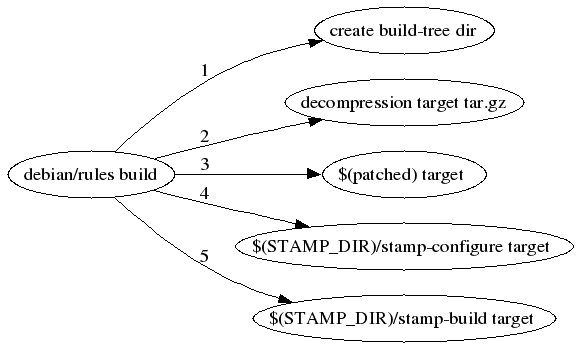
\includegraphics{image200702/dbs00.png}

\begin{enumerate}
\item create build-tree ディレクトリ \\
	\$BUILD\_TREE で指定されたディレクトリを作成します。
	デフォルトでは {\bf build-tree} になっています。

\item decompression tar.gz \\
	ソースコードが圧縮されている tar.gz を build-tree ディレクトリに解凍します。

\item \$(patched) target  \\
	debian/patches ディレクトリにあるパッチを適用します。

\item \$(STAMP\_DIR)\/stamp-configure target \\
	stamp-configure ターゲットを実行します。
	hello-dbs では \$BUILD\_TREE ディレクトリに移動し、configure を実行します。

\item \$(STAMP\_DIR)/stamp-build target \\
	stamp-build ターゲットを実行します。
	hello-dbs では \$BUILD\_TREE ディレクトリに移動し、make を実行します。 
\end{enumerate}

build 時の dpatch との違いは、

\begin{itemize}
\item パッチを当てるためのターゲット名が異なる

	dbs は \$(patched)、dpatch は patch-stamp。\\
	\$(patched) は {\bf /usr/share/dbs/dbs-build.mk}内で \$(STAMP\_DIR)/patchapply と宣言されています。

\item マーク用のファイル名が異なる

	stamp-configure や stamp-build というマーク用のファイル名が逆だったりします。
	( 通常は configure-stamp / build-stamp )
\end{itemize}


\subsubsection{パッケージのclean}
dbs の ソースのcleanターゲットはいたってシンプルです。
dpatch は 既に展開されているソースにパッチを適用するため、cleanターゲット時には適用されたパッチを外す処理が必
要になりますが、dbs では、build 時に生成されたマークファイル用ディレクトリやソース格納先ディレクトリ
(\$BUILD\_TREE)をばっさり削除します。これには、適用されたパッチの管理等を行わずに済むというメリットがあります。

しかし、dbs は パッケージビルド毎に 
\begin{enumerate}
	\item ディレクトリを削除
	\item tar.gz を解凍
	\item パッチ適用
\end{enumerate}
とするので、サイズの大きい tar.gz をパッケージ化するときは時間がかかるというデメリットもあります。

\subsection{パッチの変更}
dbs でパッチの変更を行うために以下のコマンドが提供されています。
\subsubsection{dbs-edit-patch}
	このコマンドは現在のソースからパッチを作成する環境を構築してくれます。
	hello-dbs で新しいパッチを作りたいという状況になったとします。
	以下のコマンドを実行します。

\begin{commandline}
% dbs-edit-patch  01mogeri_patch
\end{commandline}

	実行すると /tmp ディレクトリに 01mogeri\_patch というディレクトリが作成されます。
	ディレクトリの中は以下のようになっています。

\begin{commandline}
% ls -l /tmp/01mogeri_patch/
-rwxr-xr-x 1 iwamatsu iwamatsu  546 2007-02-15 06:00 dbs-update-patch
drwxr-xr-x 2 iwamatsu iwamatsu 1024 1996-08-04 23:48 hello-1.3.orig
drwxr-xr-x 2 iwamatsu iwamatsu 1024 1996-08-04 23:48 hello-1.3.orig-old
\end{commandline}

	hello-1.3.orig は修正対象のディレクトリで、hello-1.3.orig-old は修正前のディレクトリです。
	hello-1.3.orig を修正した内容と hello-1.3.orig-old で差分を取り、
	パッチを生成し、パッチをコピーしてくれるスクリプトが dbs-update-patch になっています。
	
\begin{commandline}
#!/bin/sh -e
cd "/tmp/01mogeri_patch"
HOOK_DIR=/home/iwamatsu/dev/debian/dbs/hello-dbs-1.3/debian/dbs-hooks
test -d "$HOOK_DIR" && run-parts "$HOOK_DIR" --arg update-patch-prediff
find -name "*.bak" -print0 | xargs -0 --no-run-if-empty rm
find -name "*~" -print0 | xargs -0 --no-run-if-empty rm
: > new_patch
diff -ruN  hello-1.3.orig-old hello-1.3.orig >> new_patch || test $? -eq 1
mv new_patch "/home/iwamatsu/dev/debian/dbs/hello-dbs-1.3/debian/patches/01mogeri_patch"
test -d "$HOOK_DIR" && run-parts "$HOOK_DIR" --arg update-patch-postdiff
\end{commandline}
	
	例えば、


\begin{commandline}
cat  /tmp/01mogeri_patch/hello-1.3.orig/MOGERI
mogemogeri
\end{commandline}

	という修正を行い、{\bf /tmp/dbs-update-patch} を実行した場合、

\begin{commandline}
% /tmp/01mogeri_patch/dbs-update-patch
% ls -l debian/patches/01mogeri_patch
-rw-r--r-- 1 iwamatsu iwamatsu 212 2007-02-15 06:08 debian/patches/01mogeri_patch
% cat debian/patches/01mogeri_patch
diff -ruN hello-1.3.orig-old/MOGERI hello-1.3.orig/MOGERI
--- hello-1.3.orig-old/MOGERI   1970-01-01 09:00:00.000000000 +0900
+++ hello-1.3.orig/MOGERI       2007-02-15 06:06:54.000000000 +0900
@@ -0,0 +1 @@
+mogemogeri
\end{commandline}

	となります。

\subsection{まとめ}
今回、dbs を触ってみたのですが、
\begin{itemize}
	\item ソースが見えない

		ソースが tar で固まっているため、見ることができない。
		見るには コマンドを使って解凍する必要がある。

	\item dpatch と比べてソースの編集がしずらい

		コマンドは用意されているんだけど、一回 tmp等に持っていって修正して.... という
		作業が発生するので、めんどうくさいところがある。

\end{itemize}
	という感想です。また、dbs を使っていたパッケージも だんだん dpatch に移行しつつあるので
	もう役目は追えたのではないかという気もします。

\dancersection{次回}{}

未定です。
内容は本日決定予定です。

参加者募集はまた後程。

\cleartooddpage

\begin{minipage}[b]{0.2\hsize}
 \definecolor{titleback}{gray}{0.9}
 \colorbox{titleback}{\rotatebox{90}{\fontsize{80}{80} {\gt デビアン勉強会} }}
\end{minipage}
\begin{minipage}[b]{0.8\hsize}

\vspace*{15cm}
\hrule
\vspace{2mm}

\includegraphics[width=2cm]{image200502/openlogo-nd.eps}
\noindent \Large \bf Debian 勉強会資料\\ \\
\noindent \normalfont \debmtgyear{}年\debmtgmonth{}月\debmtgdate{}日 \hspace{5mm}  初版第1刷発行\\
\noindent \normalfont 東京エリア Debian 勉強会 (編集・印刷・発行)\\
\hrule
\end{minipage}

\end{document}
